\documentclass[11pt, table]{beamer}
%\usepackage[table,x11names]{xcolor}
\usepackage[utf8]{inputenc}
\usepackage[T1]{fontenc}
\usepackage{multirow}
\usepackage{calc}
\usepackage{array}
\usepackage{graphicx}
\usepackage{multirow}

\newcommand{\p}{\pause}


\usetheme{default}

\newcommand\MyBox[2]{
	\fbox{\lower0.75cm
		\vbox to 1.7cm{\vfil
			\hbox to 1.7cm{\hfil\parbox{1.4cm}{#1\\#2}\hfil}
			\vfil}%
	}%
}

\begin{document}
	%\author{}
	\title{Introduction to Logistic Regression}
	%\subtitle{}
	%\logo{}
	%\institute{}
	%\date{}
	%\subject{}
	%\setbeamercovered{transparent}
	%\setbeamertemplate{navigation symbols}{}
	\begin{frame}[plain]
	\maketitle
\end{frame}

\begin{frame}
\frametitle{Logistic Regression}
\textbf{Example:} Duchenne Muscular Dystrophy (DMD)
\begin{itemize}
	\item Genetically-transmitted disease
	\item Passed from a mother to her children
	\item Female offspring suffer no apparent symptoms, but male offspring with the disease die at a young age.
	\item Female carriers tend to exhibit elevated levels of certain serum enzymes or proteins.
\end{itemize}
\vspace{0.1in}

Let's say we want to build a model which takes as input the serum levels and outputs our prediction about whether or not a female is a carrier.
\end{frame}

\begin{frame}
\frametitle{Logistic Regression}

We can start be doing some exploratory analysis.

\begin{center}
	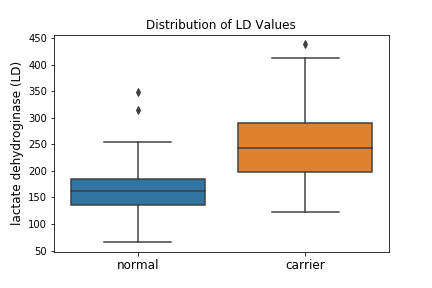
\includegraphics[width = 3in]{images/Dystrophy/LD_box.png}
\end{center}

What we can see is that in our datset, carriers tend to have higher LD values. However, there is some overlap between carriers and non-carriers in the middle values. There is not a single cutoff we can use to classify a person as a carrier or non-carrier.
\end{frame}

\begin{frame}
\frametitle{Logistic Regression}

Here is another view of the data, using a scatterplot

\begin{center}
	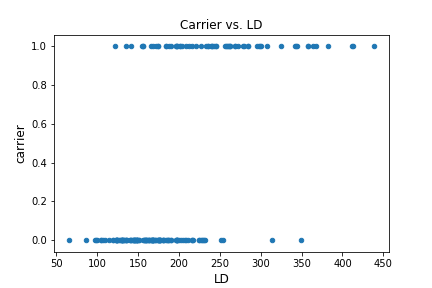
\includegraphics[width = 3in]{images/Dystrophy/scatter_01.png}
\end{center}

Here, we have encoded whether a person is a carrier or not using a numeric 0/1 value. A value of 1 indicates that a person is a carrier. 
\end{frame}


\begin{frame}
\frametitle{Logistic Regression}
Since there is overlap between carriers and non-carriers, we would probably be best off to not just make a simple prediction of carrier/non-carrier, but instead predict the likelihood or probability that a female is a carrier.
\vspace{0.1in}

From what we have seen in the plots, females with higher LD values look more likely to be carriers that those with lower values.
\vspace{0.1in}

 Between 175 and 225, it is not clear if a person is a carrier or not, so we might be best off assigning a probability close to 0.5 for people in that range.
\end{frame}

\begin{frame}
\frametitle{Logistic Regression}
So how do we create our model? We can try using a linear regression model.\p
\vspace{0.1in}

A linear regression model produces the following result:
$$\text{P(carrier)} = 0.00426\cdot(\text{LD}) - 0.4829$$

\begin{center}
	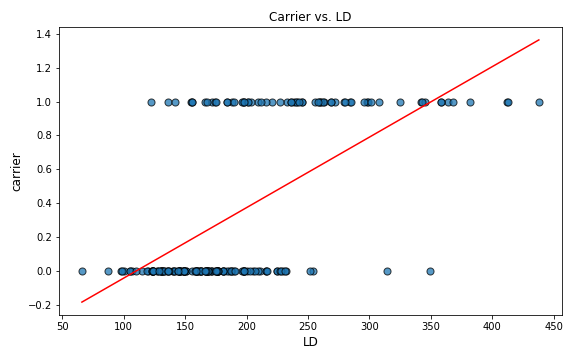
\includegraphics[width = 3in]{images/Dystrophy/scatter_02.png}
\end{center}
\end{frame}

\begin{frame}
\frametitle{Logistic Regression}
This approach has a big problem: probabilities are values between 0 and 1, but this equation has guarantee of outputting values between 0 and 1.
\vspace{0.1in}

In fact, we can see that for some values, we get predictions less than 0 or greater than 1.
\vspace{0.1in}

Another problem is that it assumes a fixed change in LD will have a fixed effect on the probability. That is, a change from 60 to 70 will have the same impact as a change from 250 to 260.
\end{frame}

\begin{frame}
\frametitle{Logistic Regression}
One possible solution to this problem is to "squash" our output between 0 and 1.
\vspace{0.1in}

A common way to do this is to pass the output from a linear model into the \textbf{logistic function}:
$$l(x) = \frac{1}{1 + e^{x}}$$

\begin{center}
	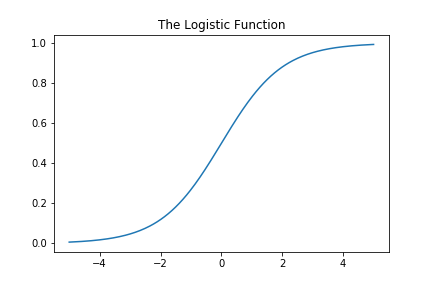
\includegraphics[width = 3in]{images/Dystrophy/logistic.png}
\end{center}
\end{frame}

\begin{frame}
\frametitle{Logistic Regression}
This means that instead of our model looking like
$$\text{P(carrier)} = \beta_1\cdot(\text{LD}) + \beta_0$$

it will look like
$$\text{P(carrier)} = \frac{1}{1 + e^{-(\beta_1\cdot(\text{LD}) + \beta_0)}}$$
\end{frame}

\begin{frame}
\frametitle{Logistic Regression}
Fitting this model, we obtain
$$\text{P(carrier)} = \frac{1}{1 + e^{-(0.02905\cdot(\text{LD}) - 6.407)}}$$
\begin{center}
	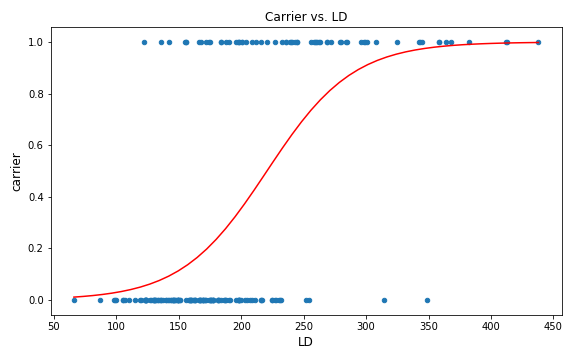
\includegraphics[width = 3in]{images/Dystrophy/scatter_03.png}
\end{center}

\end{frame}
\end{document}
